% !TEX root = main.tex
\renewcommand{\labelenumi}{\alph{enumi})}

\textbf{c. ¿Cu\'al es la probabilidad de que el proyecto finalice
despues de 13 d\'ias?}

$P(x > 13)$

\text{Si usamos las propiedades de complemento tenemos que: }

$P(x > 13) = 1 - P(x \leq 13)$

y esto es igual a $1 - P(x \leq 13) = 1 - Fx(13)$

por el inciso anterior tenemos que $Fx(13) = 0.9$ por lo tanto

$P(x>13) = 1-F(13)= 1 - .9 = .1$


\textbf{3. Un experimento aleatorio consiste en lanzar un dado equilibrado. 
Hasta obtener 6 veces el numero 6, no necesariamente de forma consecutiva.
Encuentra la probabilidad de que el experimento requiera 17 lanzamientos}
\\ \\
Ya que nosotros queremos saber la probabilidad de que en el lanzamiento 
17 se acabe el experimento por lo que en los 16 lanzamientos anteriores 
nos tiene que haber salido 5 veces 6 por lo que podemos usar la binomeal
neagtiva por lo que sea

$r =$ numero de exitos 

$p =$ prueba de exito

$x \sim $ Binhey(r,p)
\\
Entonces podemos ver que tenemos $r=6$ y $p= \frac{1}{6}$

$fx(x) = (\frac{r + x-1}{x})p^{r}(1-p)^{x}$

$f(11) = (\frac{6 + 11-1}{11})(\frac{1}{6})(1-\frac{1}{6}) = 
(\frac{16}{11})(\frac{1}{6})^{6}(\frac{5}{6})^{11} = \frac{16!}{(16-11)!11!}(\frac{1}{6}^{6})(\frac{5}{6}^{11})
= 0.1260031553$

\textbf{4. Suponga que el n\'umero de accidentes al d\'ia que ocurren en una 
parte de una carretera es una variable aleatoria Poisson por diametro $\lambda = 3$}

a) Calcule la probabilidad de que ocurran 2 o m\'as accidentes en un d\'ia cualquiera
queremos saber $P(x\leq 2)$ por las propiedades de complemento tenemos que

$P(x \leq 2)=1 -P(x<2)$

pero ya que s\'olo podemos tener n\'umeros enteros de accidenters entonces tenemos que

$P(x \geq 2)= 1-P(x<2)=1-P(x \leq 1)=1-P(x=0)-P(x=1)$

donde $fx(x)=e^{-\lambda}\frac{\lambda^{x}}{x!}\rightarrow fx(x)=e^{-3}(\frac{3^{x}}{x!})$

$1-P(x-0)-P(x=1)=1-(e^{-3}\frac{3^{0}}{0!})-(e^{-3}\frac{3^{1}}{1!}) = 0.80085172$

b) Calcule la probabilidad de que ocurran 2 o m\'as accidentes dado que ha ocurrido
al menos un accidente.

$P(x \geq 2 | x \geq 1) = \frac{P(x \geq 2 \land x \geq 1)}{P(x \geq 1)} = 
\frac{P(x \geq 2)}{P(x \geq 1)}$

Sabemos que por el inciso anterior que $P(x \geq 2) = 0.80085172$ ahora vemos que:

$P(x \geq 1)=1-P(x<1) = 1-P(x \leq 0) = 1-P(x=0) = 1-(e^{-3}(\frac{3^{0}}{0!})) = 0.95021293$

$\frac{P(x \geq 2)}{P(x \geq 1)} = \frac{0.80085172}{0.95021293} = 0.84281290$
% 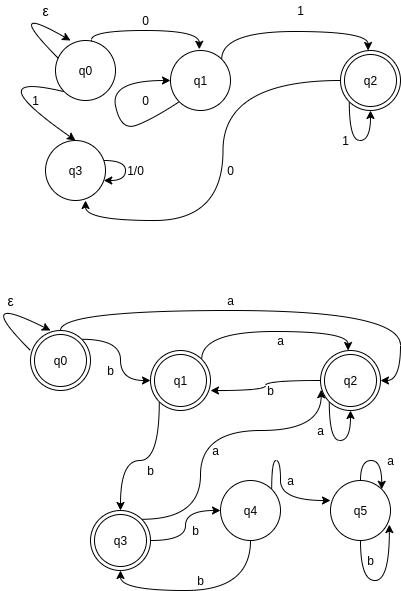
\includegraphics{semanal4.png}